%%%% SIGNAL SECTION %%%%
\section{MCS Performance on Truth-Selected Muons from numuCC Events in Simulation}\label{MCBNBRecoTrack_performance_section}

\subsection{Input sample}\label{MCBNBRecoTrack_input_sample_section}
The input sample to this portion of the analysis is roughly 800,000 MCC7 simulated BNB neutrino interactions without any cosmics simulated. These simulated events are run through a fully automated reconstruction chain and then truth information is used to select muons from numuCC interactions which are eligible for MCS analysis. The SAM definition used for this sample is ``prodgenie\_bnb\_nu\_uboone\_mcc7\_reco2''.

\subsection{Event selection}\label{MCBNBRecoTrack_eventselection_section}
The event selection for this subanalysis is truth based. The cuts are:
\begin{itemize}
\item There is one neutrino interaction in the event.
\item The neutrino interaction is of type numu charged-current, and occurs within the fiducial volume.
\item The {\sc MCTrack} associated with the outgoing muon from the interaction is fully contained within the fiducial volume.
\item The {\sc MCTrack} associated with the outgoing muon from the interaction is at least one meter in length.
\item There is a reconstructed track that starts within 3 cm of the start and ends within 3 cm of the end of the aforementioned {\sc MCTrack} (or vice-versa). This cut is requiring that the track is well reconstructed in terms of position (direction is taken into account later).
\end{itemize}
After these additional cuts are placed, 13810 events (tracks) remain for MCS analysis.



\subsection{MCS Momentum Validation}\label{MCS_Momentum_Validation_MCBNBRecoTrack_section}
For this sample of reconstructed tracks, only the 3D trajectory points of each reconstructed track are used as input to the MCS code, described in Section \ref{MCS_technique_section}. The resulting MCS momentum versus range-based momentum without any cuts other than those described in Section \ref{MCBNBRecoTrack_eventselection_section} can be seen in Figure \ref{MCS_range_momentum_MCBNBRecoTrack_fig}. \\

In order to compute a bias and a resolution, Figure \ref{MCS_range_momentum_MCBNBRecoTrack_fig} is sliced in bins of range momentum and a histogram of the fractional momentum difference ($\frac{p_{MCS}^{-1} - p_{range}^{-1}}{p_{range}^{-1}}$) is created for each bin. Note that the inverse of the momentum is used rather than the momentum because this distribution is more gaussian distributed. Also note that this fractional momentum difference using inverse of momentum is algebraically equivalent to ($\frac{p_{range} - p_{MCS}}{p_{MCS}}$). This distribution is shown for three representative bins in Figure \ref{MCS_range_bias_resolution_MCBNBRecoTrack_slices_fig}, along with the gaussian fit to each.  The mean ($\mu$) of each gaussian fit is used to compute a bias as a function of range momentum, while the width ($\sigma$) of each distribution is used to compute a resolution. The bias and resolution for this momentum reconstruction method shown in Figure \ref{MCS_range_bias_resolution_MCBNBRecoTrack_fig}. This figure indicates a bias in the MCS momentum resolution on the order of a few percent, with a resolution that decreases from about 9\% for contained tracks with true total momentum around 0.5 GeV (which corresponds to a length of about 1.7 meters) to below 7\% for contained tracks with true total momentum greater than 0.8 GeV (which corresponds to a length of about 3.1 meters). This agrees reasonably well with the analogous plots created from simulated single muons with {\sc MCTracks} (Figure \ref{MCS_range_bias_resolution_MCTrack_fig}).


\begin{figure}[ht!]
\begin{center}
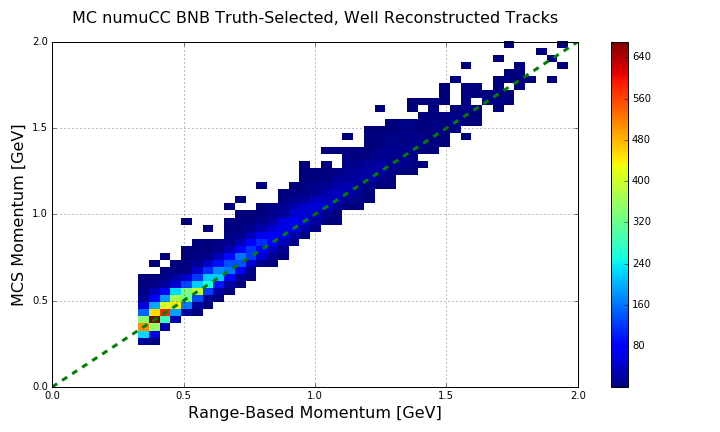
\includegraphics[width=100mm]{Figures/MCS_range_comparison_MCBNBRecoTrack.png}
\end{center}
\caption{\textit{MCS computed momentum versus range momentum for the truth-selected simulated fully contained, well reconstructed muon tracks from numu charged current events.}}
\label{MCS_range_momentum_MCBNBRecoTrack_fig}
\end{figure}


\begin{figure}
\centering
\mbox{
	\subfigure[\textit{Fractional momentum difference between 0.35 and 0.53 GeV range momentum.}]
	{\includegraphics[width=50mm]{Figures/{MCS_range_resolution_MCBNBRecoTrack_slice_0.35_0.53}.png}}
	\quad
	\subfigure[\textit{Fractional momentum difference between 0.90 and 1.08 GeV range momentum.}]
	{\includegraphics[width=50mm]{Figures/{MCS_range_resolution_MCBNBRecoTrack_slice_0.90_1.08}.png}}
	\quad
	\subfigure[\textit{Fractional momentum difference between 1.45 and 1.63 GeV range momentum.}]
	{\includegraphics[width=50mm]{Figures/{MCS_range_resolution_MCBNBRecoTrack_slice_1.45_1.63}.png}}
	}

\caption{\textit{Fractional momentum difference for a few representative bins of range momentum derived from Figure \ref{MCS_range_momentum_MCBNBRecoTrack_fig}.}}
\label{MCS_range_bias_resolution_MCBNBRecoTrack_slices_fig}
\end{figure}


\begin{figure}
\centering
\mbox{
	\subfigure[\textit{MCS momentum bias as a function of range momentum.}]
	{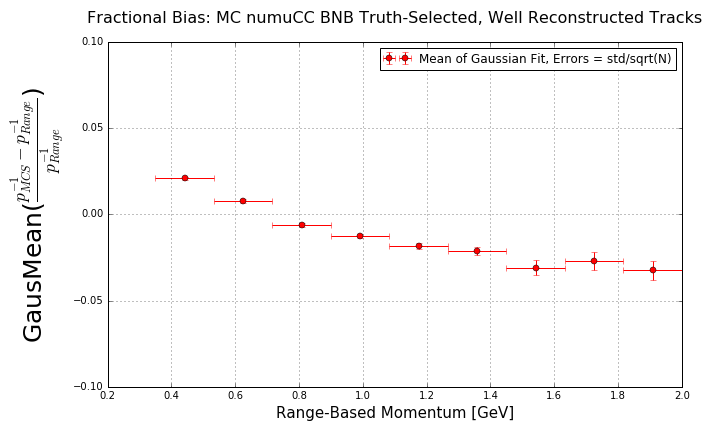
\includegraphics[width=75mm]{Figures/MCS_range_bias_MCBNBRecoTrack.png}}
	\quad
	\subfigure[\textit{MCS momentum resolution as a function of range momentum.}]
	{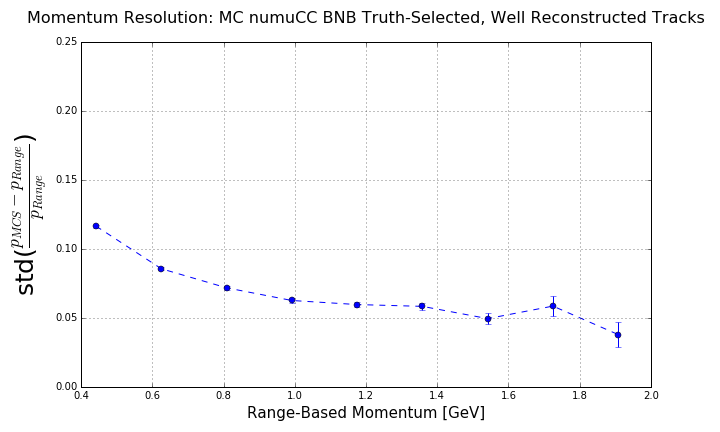
\includegraphics[width=75mm]{Figures/MCS_range_resolution_MCBNBRecoTrack.png}}
	}
\caption{\textit{MCS momentum bias and resolution as a function of range momentum for the truth-selected simulated fully contained, well reconstructed muon tracks from numu charged current events.}}
\label{MCS_range_bias_resolution_MCBNBRecoTrack_fig}
\end{figure}



\subsection{Highland Validation}\label{Highland_Validation_MCBNBRecoTrack_section}
For this sample of tracks, the same Highland validation plot is created in exactly the same way as described in Section \ref{Highland_Validation_MCTrack_section}. For each consecutive pair of segments, the angular scatter in milliradians divided by the Highland expected RMS in millradians is an entry in the histogram shown in Figure \ref{Highland_validation_MCBNBRecoTrack_fig}. From this figure we can see that the Highland formula is valid for well reconstructed tracks in simulation when 10 cm segments are used.

\begin{figure}[ht!]
\begin{center}
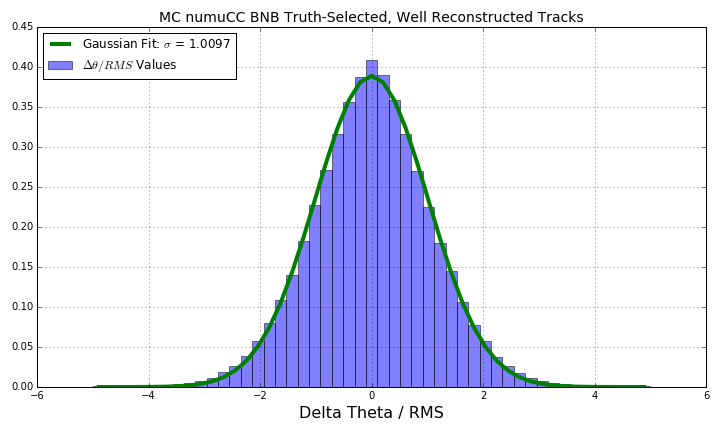
\includegraphics[width=100mm]{Figures/Highland_validation_MCBNBRecoTrack.png}
\end{center}
\caption{\textit{10 cm segment angular deviations divided by expected Highland RMS for the sample of well reconstructed, neutrino induced muons in simulation.}}
\label{Highland_validation_MCBNBRecoTrack_fig}
\end{figure}


\subsection{Optimizing Segment Length}\label{SegmentLength_MCBNBRecoTrack_section}
One of the tunable parameters in the MCS algorithm is the length of segments into which a track is broken. While shorter segment lengths yield more segments per track and therefore more sampling points to build a stronger likelihood, they also lead to the breakdown of the gaussian nature of scatters. Longer segments tend to have a more gaussian distribution of scatters but lead to fewer sampling points and therefore worse momentum resolution. Additionally, shorter segment lengths tend to have a higher momentum bias. For these reasons there exists an optimal segment length. Figure \ref{Highland_seglenstudy_MCBNBRecoTracks_fig} shows analogous figures to Figure \ref{Highland_validation_MCBNBRecoTrack_fig} for four different segment lengths ranging between 2 cm and 20 cm, with the same input sample of tracks. From this figure it can be seen that only segment lengths longer than or equal to 10 cm provide truly gaussian distributions.\\
Figure \ref{seglenstudy_bias_resolution_MCBNBRecoTrack_fig} shows the bias and resolution for the MCS momentum reconstruction method on this same sample. Here we see that shorter segment lengths tend to have a higher bias. Similarly, shorter segment lengths tend to have better resolution but the difference is small at larger range momenta. For range momenta below about 0.5 GeV the difference in resolution between segment lengths grows because the tracks are short enough where the longer segment lengths are not providing enough sampling points for the MCS method to make an accurate estimation of the track momentum. In order to maintain a gaussian distribution of angular scatters while providing enough sampling points for an momentum resolution of below 10\% for the shortest viable tracks, a segment length of 10 cm has been chosen for this analysis.

\begin{figure}
\centering
\mbox{
	\subfigure[\textit{Highland validation figure for 2 cm segment lengths.}]
	{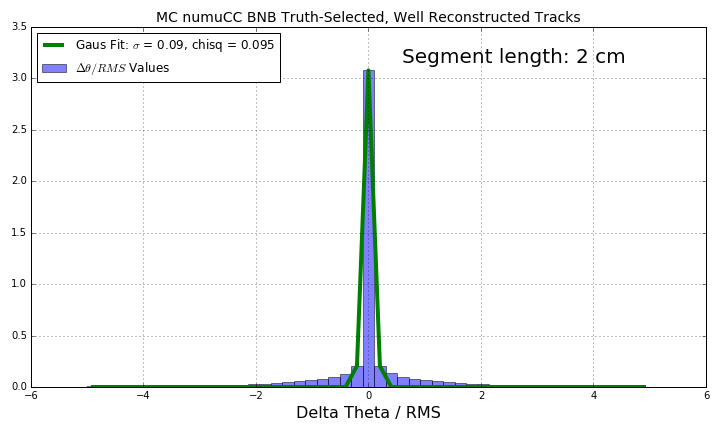
\includegraphics[width=75mm]{Figures/seglenstudy_gaus_2cm.png}}
	\quad
	\subfigure[\textit{Highland validation figure for 5 cm segment lengths.}]
	{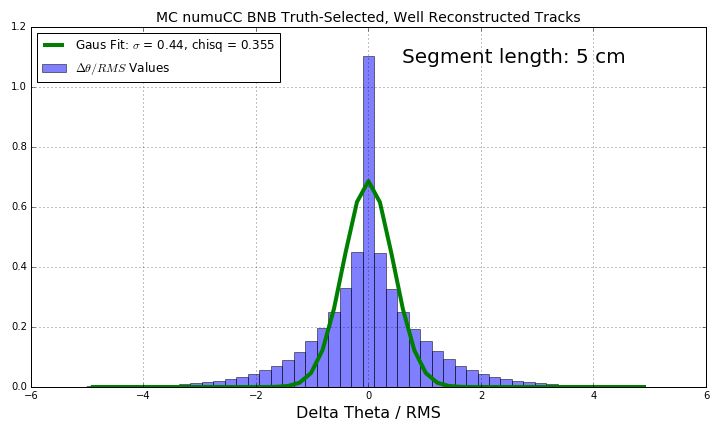
\includegraphics[width=75mm]{Figures/seglenstudy_gaus_5cm.png}}
	}\newline
\mbox{
	\subfigure[\textit{Highland validation figure for 10 cm segment lengths.}]
	{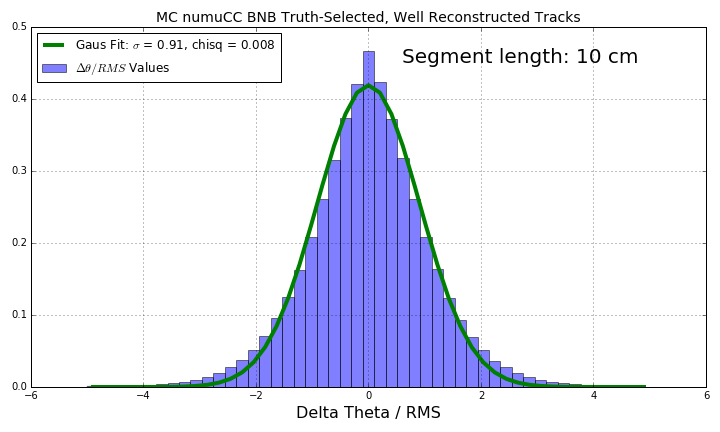
\includegraphics[width=75mm]{Figures/seglenstudy_gaus_10cm.png}}
	\quad
	\subfigure[\textit{Highland validation figure for 20 cm segment lengths.}]
	{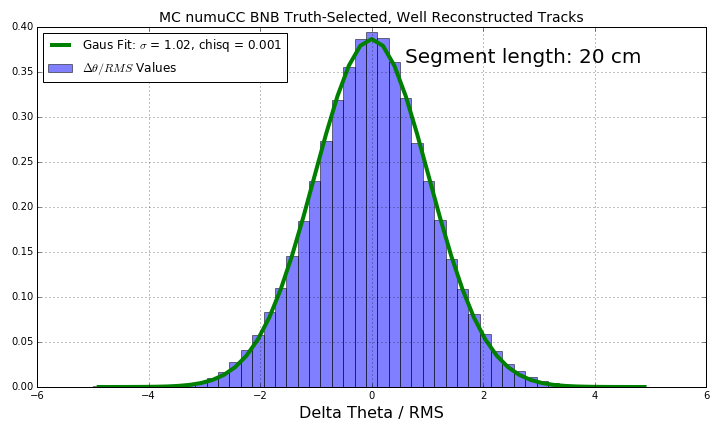
\includegraphics[width=75mm]{Figures/seglenstudy_gaus_20cm.png}}
	}
\caption{\textit{Highland validation figures analogous to Figure \ref{Highland_validation_MCBNBRecoTrack_fig} for various segment lengths, taken from the sample of well reconstructed neutrino-induced truth-selected muons in simulation. The gaussian nature of this plot breaks down for segment lengths that are too short.}}
\label{Highland_seglenstudy_MCBNBRecoTracks_fig}
\end{figure}



\begin{figure}
\centering
\mbox{
	\subfigure[\textit{MCS momentum bias as a function of range momentum for four different segment lengths.}]
	{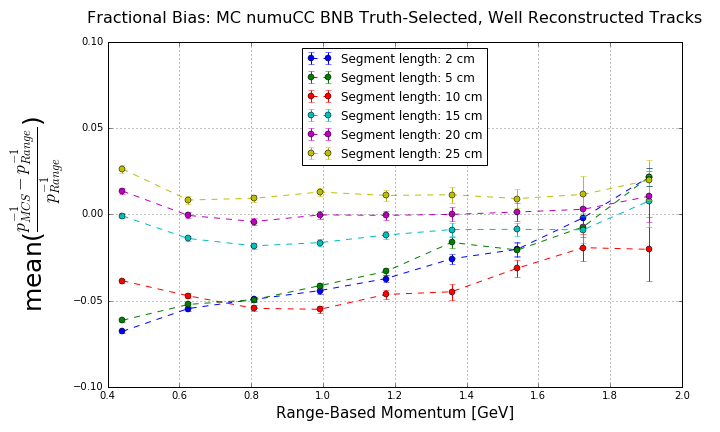
\includegraphics[width=75mm]{Figures/seglenstudy_MCBNBRecoTrack_bias.png}}
	\quad
	\subfigure[\textit{MCS momentum resolution as a function of range momentum for four different segment lengths.}]
	{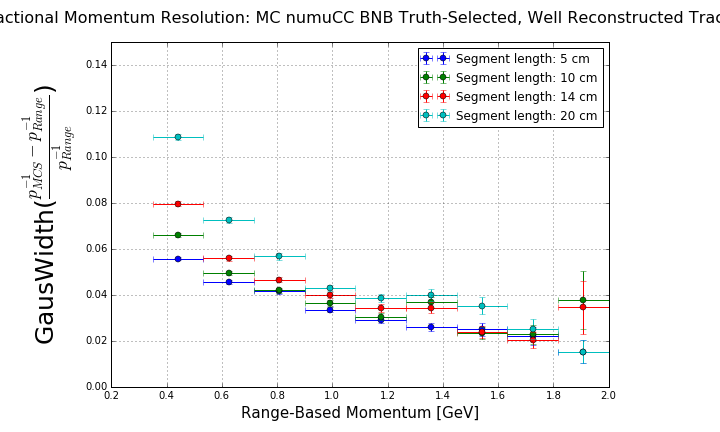
\includegraphics[width=75mm]{Figures/seglenstudy_MCBNBRecoTrack_resolution.png}}
	}
\caption{\textit{MCS momentum bias and resolution as a function of range momentum for the selected, well reconstructed neutrino-induced truth-selected muons in simulation.}}
\label{seglenstudy_bias_resolution_MCBNBRecoTrack_fig}
\end{figure}



\subsection{Optimizing Constant Detector Resolution Term}\label{ResolutionStudy_MCBNBRecoTrack_section}
This section describes how the resolution term $\sigma_\theta^{res}$ in the modified Highland equation, Equation \ref{modified_highland_eqtn} is chosen. This constant was chosen \textit{after} choosing the optimal segment length of 10 cm described in Section \ref{SegmentLength_MCBNBRecoTrack_section}. In order to choose a resolution term, a procedure similar to the one described in the segment length optimization section (Section \ref{SegmentLength_MCBNBRecoTrack_section}). This sample of well-reconstructed truth-selected muons from numu charged current interactions in simulation was analyzed with various different resolution terms. It was found that the resolution term has a very small impact for the muons studied in this sample. It is worth noting that this resolution term will have a stronger impact on the energy resolution the higher energy the muons are (as higher energy muons have smaller angular scatters so the resolution term begins to dominate), but since this study only considers contained muons that have lower energy, the term's impact is weak.\\

The momentum bias and resolution are computed in the usual way for different resolution terms, using the nominal 10 cm segment length in the algorithm. The results can be seen in Figures \ref{ResolutionStudy_MCBNBRecoTrack_bias_fig} and \ref{ResolutionStudy_MCBNBRecoTrack_resolution_fig} respectively. For 10 cm segments, the resolution terms have small impact on the bias and momentum resolution of the algorithm so long as the resolution parameter isn't exceedingly large (above 5 mrad). Therefore, a default resolution of 2 mrad has been chosen to be used for the entirety of this analysis.

\begin{figure}
\centering
\mbox{
	\subfigure[\textit{MCS momentum bias as a function of range momentum for five different resolution terms.}\label{ResolutionStudy_MCBNBRecoTrack_bias_fig} ]
	{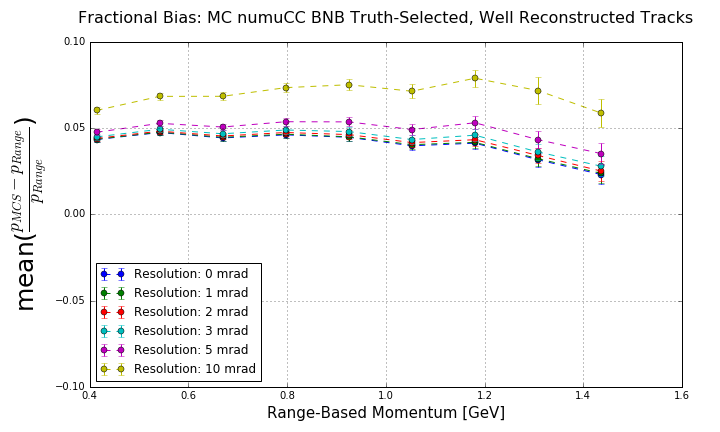
\includegraphics[width=75mm]{Figures/resstudy_MCBNBRecoTrack_bias.png}}
	\quad
	\subfigure[\textit{MCS momentum resolution as a function of range momentum for five different resolution terms.}\label{ResolutionStudy_MCBNBRecoTrack_resolution_fig} ]
	{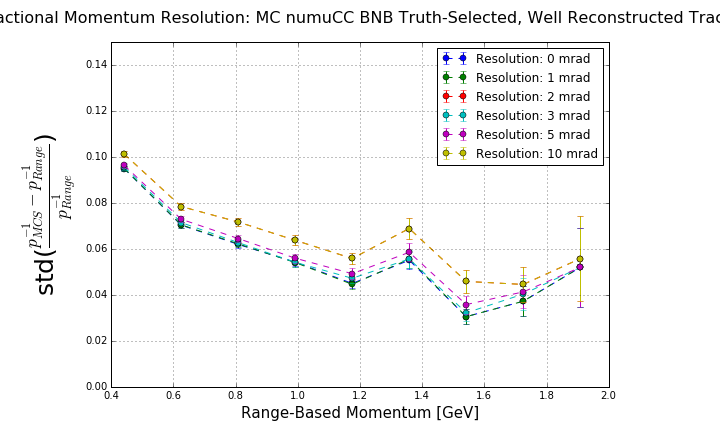
\includegraphics[width=75mm]{Figures/resstudy_MCBNBRecoTrack_resolution.png}}
	}
\caption{\textit{The impact of constant resolution terms, $\sigma_\theta^{res}$ in the modified Highland equation, Equation \ref{modified_highland_eqtn}.}}
\end{figure}


\subsection{MCS to Determine Track Direction}\label{TrackDirection_MCBNBRecoTrack_section}
This section demonstrates the ability for the multiple coloumb scattering algorithm to determine the direction of a track. The MCS code as it is described in Section \ref{MCS_technique_section} works by maximizing a likelihood based on angular scatters between segments of a track along with the expected RMS angular deviation from the modified Highland equation (Equation \ref{modified_highland_eqtn}). In practice, there is actually a negative log likelihood that is minimized, meaning the lower the likelihood the more confident the fit is. In order to determine the direction of a track with MCS, one can compute the converged minimum negative log likelihood for the track assuming it is oriented in the correct direction, then reverse the ordering of the trajectory points in the track and compute the converged minimum negative log likelihood for the reversed track. The likelihood should be better (smaller) for tracks in the correct direction than their reversed counterparts.\\

Given this truth-selected sample in simulation, the true direction of the track is known. The minimized negative log likelihood for each of these tracks both in the correct (forwards) direction and incorrect (backwards) direction can be seen in Figure \ref{TrackDirection_MCBNBRecoTrack_LLHDoverlay_fig}. A smaller likelihood here means a better fit in the MCS code. Figure \ref{TrackDirection_MCBNBRecoTrack_LLHDdiff_fig} shows the difference of these two distributions, forwards minus backwards. Any negative entries in this figure indicate that the forwards-going track had a better fit than backwards-going. This figure shows that MCS can be used as a tool to test track direction.

\begin{figure}
\centering
\mbox{
	\subfigure[\textit{The minimized negative log likelihood value for each track in the well-reconstructed, fully contained neutrino-induced truth-selected muon tracks in simulation sample, both with tracks oriented in the correct (forwards) direction and reversed (backwards) direction. A smaller likelihood here means a better fit in the MCS code.}\label{TrackDirection_MCBNBRecoTrack_LLHDoverlay_fig}]
	{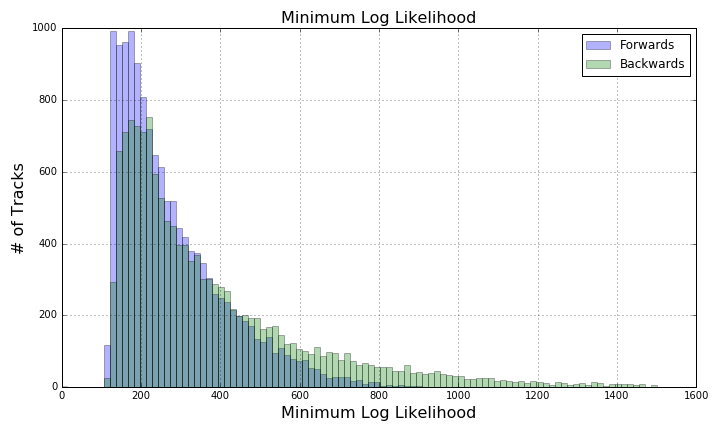
\includegraphics[width=75mm]{Figures/TrackDirection_MCBNBRecoTrack_LLHDoverlay.png}}
	\quad
	\subfigure[\textit{The difference, forwards minus backwards, of the log likelihoods. Negative entries indicate that the forwards-going tracks had a better fit than the backwards-going ones.}\label{TrackDirection_MCBNBRecoTrack_LLHDdiff_fig}]
	{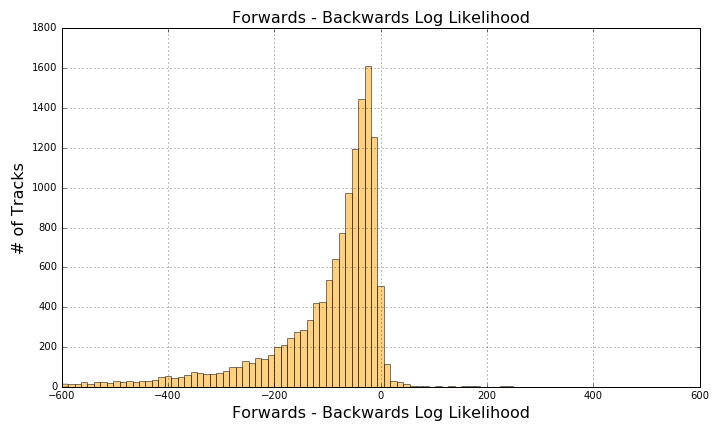
\includegraphics[width=75mm]{Figures/TrackDirection_MCBNBRecoTrack_LLHDdiff.png}}
	}
\caption{\textit{Evidence that MCS can be used to determine track directions by analyzing the output of the likelihood fit.}}
\end{figure}

